\documentclass{article}
\usepackage[utf8]{inputenc}

\title{Homework No.5}
\author{Osamu Katagiri-Tanaka : A01212611}
\date{\today}

% import math symbols
\usepackage{amsmath, esint}
\usepackage{cancel}

% import code snippets
\usepackage{listings}
\usepackage{xcolor}
\definecolor{codegreen}{rgb}{0,0.6,0}
\definecolor{codegray}{rgb}{0.5,0.5,0.5}
\definecolor{codepurple}{rgb}{0.58,0,0.82}
\definecolor{backcolour}{rgb}{0.99,0.99,0.96}
\lstdefinestyle{mystyle}{
  backgroundcolor   = \color{backcolour},
  commentstyle      = \color{codegreen},
  keywordstyle      = \color{magenta},
  numberstyle       = \tiny\color{codegray},
  stringstyle       = \color{codepurple},
  basicstyle        = \ttfamily\small,
  breakatwhitespace = false,
  breaklines        = true,
  captionpos        = b,
  keepspaces        = true,
  numbers           = left,
  numbersep         = 2pt,
  showspaces        = false,
  showstringspaces  = false,
  showtabs          = false,
  tabsize           = 2,
  aboveskip         = 0.1em,
  belowskip         = 0.1em
}
\lstset{style=mystyle}

% import hyperlinks
\usepackage{hyperref}
\hypersetup{
  colorlinks = true,
  linkcolor  = red,
  filecolor  = red,
  citecolor  = red,
  urlcolor   = red
}

% import continuous lists
\usepackage{enumitem}

% format margins and paper size
\usepackage{geometry}
\geometry{
	paper         = a4paper, % Change to letterpaper for US letter
	inner         = 2.5cm,   % Inner margin
	outer         = 2.5cm,   % Outer margin
	bindingoffset = 0.5cm,   % Binding offset
	top           = 1.5cm,   % Top margin
	bottom        = 1.5cm    % Bottom margin
}

% import figure handler
\usepackage{graphicx}

% import references handler
\usepackage[
  style     = ieee,         % references format style
  backend   = biber,        % choose the processing program
  natbib    = true,         % enable additional reference formats
  citestyle = numeric-comp, % enable multiple citations
  sortcites = true,         % sort references in multiple citations
  sorting   = nyt           % sort the reference table
]{biblatex}
\addbibresource{references.bib}

% Note that ‘d’ in the differential is conventionally set in roman.
\newcommand{\ud}{\,\mathrm{d}}

% Paragraph spacing
\setlength{\parskip}{0.2cm}           % spacing between paragraphs
\renewcommand{\baselinestretch}{1.25} % spacing between lines

\begin{document}

\maketitle

\section{Part A : Vector Field}

Matlab's \emph{quiver(X,Y,U,V)} function plots arrows with directional components $U$ and $V$ at the Cartesian coordinates specified by $X$ and $Y$. When implementing \emph{quiver}, the first arrow originates from the point $(X(1), Y(1))$, extends horizontally according to $U(1)$, and extends vertically according to $V(1)$. This function scales the arrow lengths so that they do not overlap.

On the other hand, Matlab's \emph{contour(X,Y,Z)} function creates a contour plot containing the isolines of a matrix $Z$, where $Z$ contains height values on the $x-y$ plane. \emph{contour} automatically selects the contour lines to display. $X$ and $Y$ are the $x$ and $y$ coordinates in the plane, respectively.

Listing \ref{lis:vectorFieldVisualization} implements functions \emph{quiver} and \emph{contour} to visualize the velocity field and pressure lines given a vector field. Figure \ref{img:aVectorField} is the result.

\begin{lstlisting}[language=Matlab, caption=Vector Field Visualization, label=lis:vectorFieldVisualization]
%% HW05 part A - Velocity Field, adapted from (jose lopez salinas)'s solution 
clear;
close all;

% create points to visualize
xyLim  = 2.5;
xyStep = xyLim/10;
[x, y] = meshgrid(-xyLim : xyStep : xyLim);

VectorX = cos(y); % vector in the x direction
VectorY = sin(x); % vector in the y direction

V = sqrt(VectorX.^2 + VectorY.^2);
PHI = 6 + x.^3 / 3 - y.^2 .* x - y;
[Dx, Dy] = gradient(V, 0.2, 0.2);

% Display
figure;
quiver(x, y, VectorX, VectorY);
hold on;
contour(x, y, PHI);
colorbar;
hold off;
xlabel('x-axis');
ylabel('y-axis');
title('Velocity Field, and Pressure Lines');
\end{lstlisting}

\begin{figure}[h!]
	\centering
	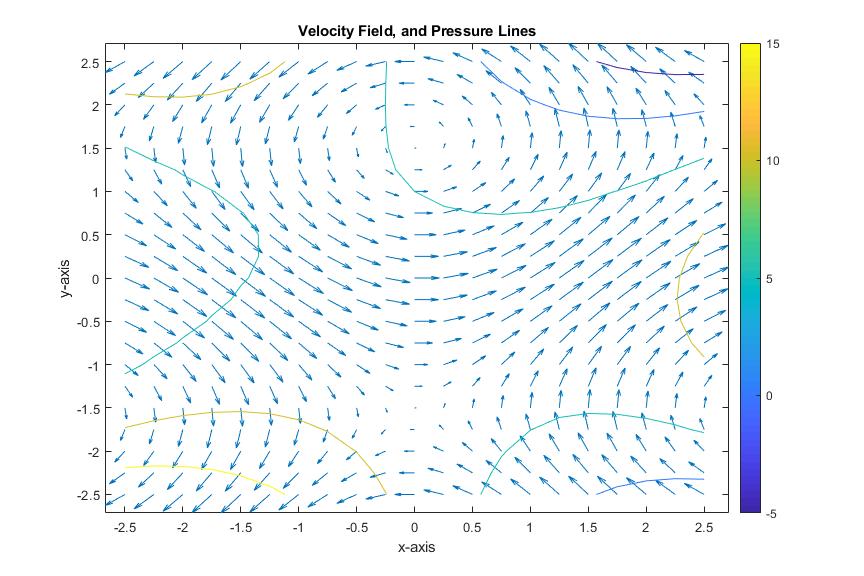
\includegraphics[width=0.90\textwidth]{./matlab/vectorField.png}
	\caption{Visualization of a Velocity Field}
	\label{img:aVectorField}
\end{figure}


\section{Part B : 1-D PDE Tubular Chemical Reactor}

The equation of conservation of chemical species under a chemical reaction of
decomposition can be represented with the PDE given below.

$$ \frac{\partial C}{\partial t} = \vec{\nabla} \cdot (D \vec{\nabla} C) - \vec{v} \cdot \vec{\nabla} C - k C^n $$

If a tubular catalytic chemical reactor initially filled with an inert solvent $(C = 0)$ is fed by a stream of component ``A" with a concentration of $1 kmol/m^3$ $(C = 1)$ and speed of $1 m/s$ $(v = 1)$, calculate the distribution of ``A" across the reactor and as a function of time $C(x, t)$. The dispersion coefficient of the component ``A" is $0.02 m^2/s$ $(D = 0.001)$, the kinetic decomposition coefficient $0.05 s^{-1}$ $(k = 1.5)$. The chemical decomposition kinetics is first order $(n = 1)$.

The molar balance in axial direction for a 1D flow can be written as:

$$ \frac{\partial C}{\partial t} = D \frac{\partial^2 C}{\partial x^2} - v \frac{\partial C}{\partial x} - k C^n $$

The initial condition $IC$ is:
$$ \left. C \right|_{t = 0} = 0 \textrm{, } 0 \leq x \leq 1 $$

The boundary conditions $BCs$ are:
$$ \left. C \right|_{x = 0} = 1 \textrm{, } t > 0 $$
$$ \left. \frac{\partial C}{\partial t} \right|_{x = L} = 0 \textrm{, } t \geq 0 $$

Where, \\
$D$ is the diffusion coefficient \\
$C$ is the injection concentration \\
$v$ is the velocity of fluid injection \\
$k$ is the first order kinetic coefficient \\
$L$ is the length of domain \\
$t$ is the simulation time \\
$x$ is the distance mesh

The PDE shall be transformed into a set of ordinary differential equations ODEs using central finite differences in space, as depicted in the central differences discretization Equation \ref{eq:reactorODEform}.

\begin{equation}
\frac{\ud C_i}{\ud t} = D \frac{C_{i+1} - 2 C_i + C_{i-1}}{\left( \Delta x \right)^2} - v \frac{C_{i+1} - C_{i-1}}{2 \Delta x} - k {C_i}^n
\label{eq:reactorODEform}
\end{equation}

Equations \ref{eq:reactorAEform_Oh2}, \ref{eq:reactorAEform_Oh3} and \ref{eq:reactorAEform_Oh4} are the backward differences discretization for $O(h^2)$, $O(h^3)$ and $O(h^4)$, respectively. Listing \ref{lis:reactorRungeKuttaODEsolver} solves the ODEs with truncation errors of $O(h^2)$, $O(h^3)$ and $O(h^4)$. \emph{ode45} results are displayed in Figures \ref{img:Oh2TruncationError}, \ref{img:Oh3TruncationError} and \ref{img:Oh4TruncationError} for which no noticeable differences can be depicted. The results from the three truncation errors as similar, as the difference between each one is around 2 percent. See Listings \ref{lis:reactorComputePercentError} and \ref{lis:reactorPercentErrorsForEachTruncation}.

\begin{equation}
\begin{aligned}
\frac{\ud C_N}{\ud x} = \frac{C_{N-2} - 4 C_{N-1} + 3 C_N}{2 \Delta x} = 0 \\
C_N = \frac{4 C_{N-1} - C_{N-2}}{3}
\end{aligned}
\label{eq:reactorAEform_Oh2}
\end{equation}

\begin{equation}
\begin{aligned}
\frac{\ud^2 C_N}{\ud x^2} = \frac{- C_{N-3} + 4 C_{N-2} - 5 C_{N-1} + 2 C_N}{\left( \Delta x \right)^2} = 0 \\
C_N = \frac{C_{N-3} - 4 C_{N-2} + 5 C_{N-1}}{2}
\end{aligned}
\label{eq:reactorAEform_Oh3}
\end{equation}

\begin{equation}
\begin{aligned}
\frac{\ud^3 C_N}{\ud x^3} = \frac{3 C_{N-4} - 14 C_{N-3} + 24 C_{N-2} - 18 C_{N-1} + 5 C_N}{2 \left( \Delta x \right)^3} = 0 \\
C_N = \frac{- 3 C_{N-4} + 14 C_{N-3} - 24 C_{N-2} + 18 C_{N-1}}{5}
\end{aligned}
\label{eq:reactorAEform_Oh4}
\end{equation}

\begin{lstlisting}[language=Matlab, caption=Reactor : Runge-Kutta ODE solver, label=lis:reactorRungeKuttaODEsolver]
%% Runge-Kutta
p(1)  = 0.001; % Diffusion coefficient D
p(2)  = 1.0;   % Injection concentration c0
p(3)  = 1.5;   % First order kinetic coefficient k
p(4)  = 1.0;   % Velocity of fluid injection vo
M     = 2*640; % Number of nodes
p(5)  = M;
Tspan = [0 1]; % Domain of time
xi    = linspace(0, 1, M);

% Initial conditions of the resulting set of ODEs
Y0    = zeros(M, 1);
Y0(1) = 1.0;

% Solve differential equation (medium order method)
% use @reactub_2 for O(h^2) truncation error
% use @reactub_3 for O(h^3) truncation error
% use @reactub_4 for O(h^4) truncation error
OPTIONS   = [];
[time_2, Y_2] = ode45(@reactub_2, Tspan, Y0, OPTIONS, p);
[time_3, Y_3] = ode45(@reactub_3, Tspan, Y0, OPTIONS, p);
[time_4, Y_4] = ode45(@reactub_4, Tspan, Y0, OPTIONS, p);

% group all data / prepare to plot ...
time     = {time_2, time_3, time_4};
Y        = {   Y_2,    Y_3,    Y_4};
Yprime   = {  Y_2',   Y_3',   Y_4'};
plotName = {'Oh2_truncationError', 'Oh3_truncationError', 'Oh4_truncationError'};
\end{lstlisting}

\begin{lstlisting}[language=Matlab, caption=Reactor : Plot the solutions, label=lis:plotTheSolutions]
% Plot limits
noOf_curvesToPlot = 10;
dlim              = 0.02;
time_lim          = [0 - dlim, 1 + dlim];
Y_lim             = [0 - dlim, 1 + dlim];
xi_lim            = [0 - dlim, 1 + dlim];
Yprime_lim        = [0 - dlim, 1 + dlim];

for plotCount = 1:1:3
    % Display concentration vs. time
    totalNoOf_curves  = size(Y{1, plotCount}, 2);
    noOf_curvesToSkip = fix(totalNoOf_curves/noOf_curvesToPlot);
    figure;
    subplot(1, 2, 1)
    for n = linspace(1, totalNoOf_curves, totalNoOf_curves)
        hold all
        if mod(n, noOf_curvesToSkip) == 0
            plot(time{1, plotCount}, Y{1, plotCount}(:, n));
        end
    end
    xlabel('time \tau');
    ylabel('Concentration mol/dm^3');
    axis([time_lim(1) time_lim(2) Y_lim(1) Y_lim(2)])

    % Display concentration vs. distance
    totalNoOf_curves  = size(Yprime{1, plotCount}, 2);
    noOf_curvesToSkip = fix(totalNoOf_curves/noOf_curvesToPlot);
    %figure;
    subplot(1, 2, 2)
    for n = linspace(1, totalNoOf_curves, totalNoOf_curves)
        hold all
        if mod(n, noOf_curvesToSkip) == 0
            plot(xi, Yprime{1, plotCount}(:, n));
        end
    end
    xlabel('distance x/L');
    ylabel('Concentration mol/dm^3');
    axis([xi_lim(1) xi_lim(2) Yprime_lim(1) Yprime_lim(2)])
end
\end{lstlisting}

\begin{figure}[h!]
	\centering
	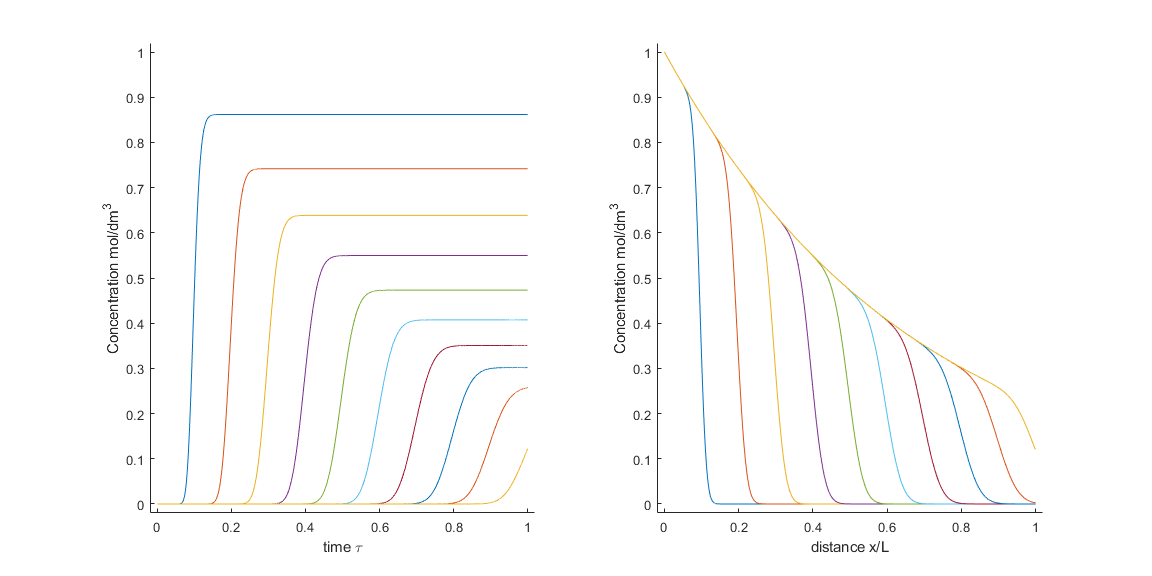
\includegraphics[width=0.90\textwidth]{./matlab/Oh2_truncationError.png}
	\caption{$O(h^2)$ Truncation Error}
	\label{img:Oh2TruncationError}
\end{figure}

\begin{figure}[h!]
	\centering
	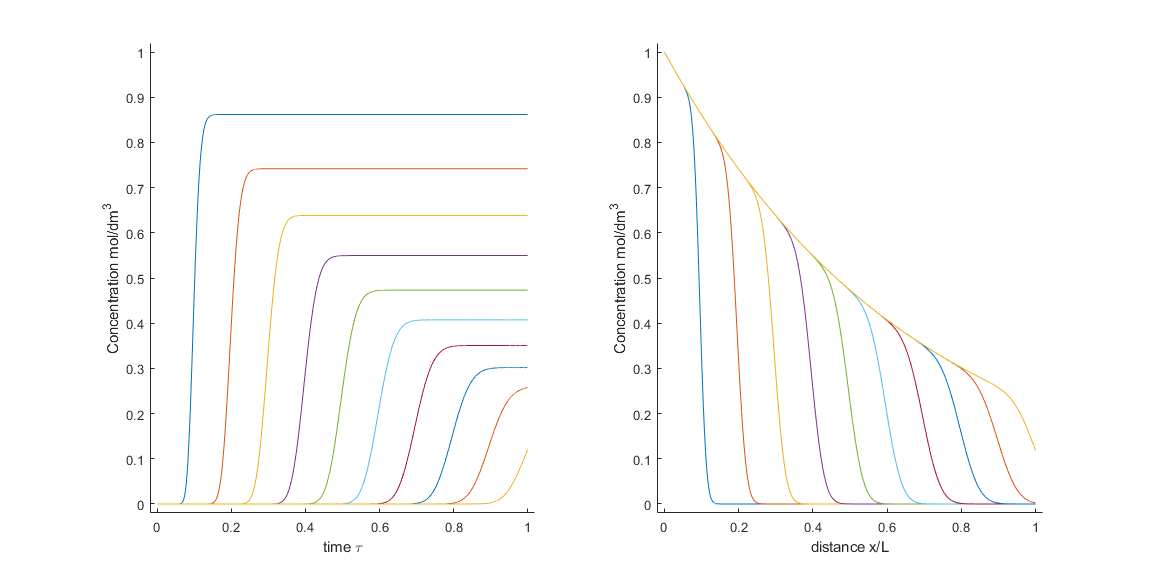
\includegraphics[width=0.90\textwidth]{./matlab/Oh3_truncationError.png}
	\caption{$O(h^3)$ Truncation Error}
	\label{img:Oh3TruncationError}
\end{figure}

\begin{figure}[h!]
	\centering
	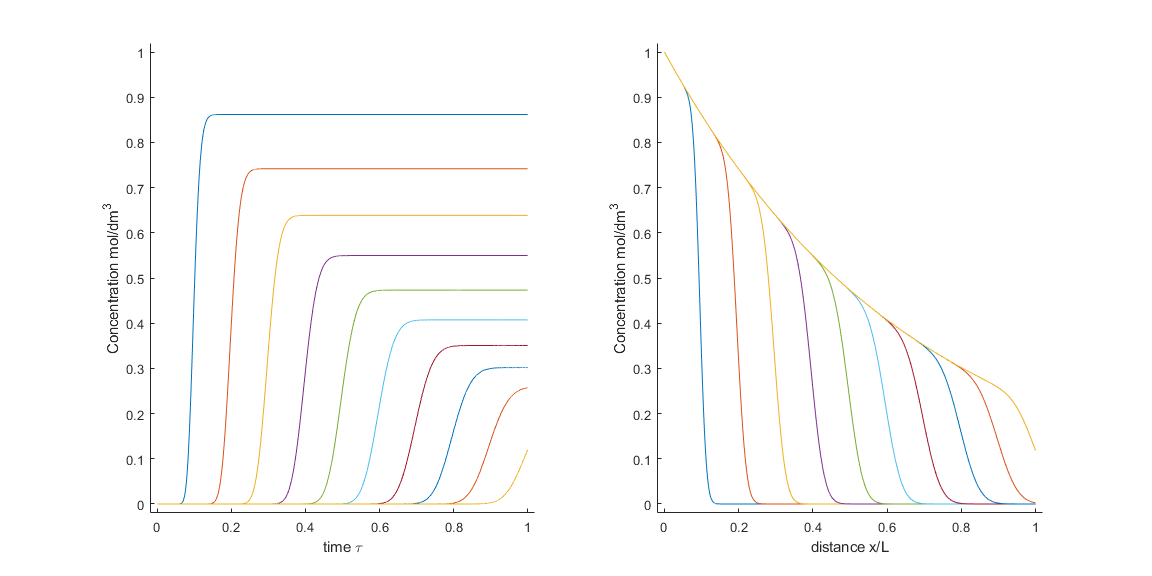
\includegraphics[width=0.90\textwidth]{./matlab/Oh4_truncationError.png}
	\caption{$O(h^4)$ Truncation Error}
	\label{img:Oh4TruncationError}
\end{figure}

\begin{lstlisting}[language=Matlab, caption=Reactor : Compute percent error for each implementation, label=lis:reactorComputePercentError]
%% Print error between O(h)s
sprintf(                                                          ...
    '(O(h^2) - O(h^3))/O(h^2)*100 error: %f%%',                   ...
    (Yprime{1, 1}(end) - Yprime{1, 2}(end))/Yprime{1, 1}(end)*100 ...
)
sprintf(                                                          ...
    '(O(h^2) - O(h^4))/O(h^2)*100 error: %f%%',                   ...
    (Yprime{1, 1}(end) - Yprime{1, 3}(end))/Yprime{1, 1}(end)*100 ...
)
sprintf(                                                          ...
    '(O(h^3) - O(h^4))/O(h^3)*100 error: %f%%',                   ...
    (Yprime{1, 2}(end) - Yprime{1, 3}(end))/Yprime{1, 2}(end)*100 ...
)
\end{lstlisting}

\begin{lstlisting}[caption=Reactor : Percent errors for each truncation, label=lis:reactorPercentErrorsForEachTruncation]
ans =
    '(O(h^2) - O(h^3))/O(h^2)*100 error: 1.908447%'
ans =
    '(O(h^2) - O(h^4))/O(h^2)*100 error: 1.919032%'
ans =
    '(O(h^3) - O(h^4))/O(h^3)*100 error: 0.010792%'
\end{lstlisting}


\section{Part C : Growing Bubbles}

The growth and collapse of bubbles is given by Equations \ref{eq:bubbleRadius}.

\begin{equation}
\begin{aligned}
\ddot{y} y + \frac{3}{2} \left( \dot{y} \right)^2 = -B(\tau) + \frac{1}{y^{3 k}}\\
\ddot{y} = \frac{\ud^2 y}{\ud \tau^2}\\
\dot{y} = \frac{\ud y}{\ud \tau}
\end{aligned}
\label{eq:bubbleRadius}
\end{equation}

Where $y$ is the ratio of the actual radius and the initial radius of the bubble. $\tau$ is the dimensionless time: $\displaystyle y = \frac{R}{R_0} $ $\displaystyle \tau = \frac{t}{R_0 \sqrt{\frac{\rho}{p_0}}}$. The initial conditions are: $\displaystyle y \rvert_{\tau = 0} = 1$ and $\displaystyle \dot{y} \rvert_{\tau = 0} = 0$

Listing \ref{lis:growingBubblesSolveAndPlot} solves the ODEs to describe the evolution of the air bubbles in time given a pressure perturbation $B(\tau)$

$$
B(\tau) =
    \begin{cases}
      \frac{1 + cos\left( \pi \frac{\tau}{5} \right)}{5} & 0 \leq \tau \leq 10\\
      1 & \text{otherwise}
    \end{cases}
$$

\begin{lstlisting}[language=Matlab, caption=Growing Bubbles : Solve and Plot, label=lis:growingBubblesSolveAndPlot]
% Runge-Kutta
% k = 1.4 adiabatic process, k = 1 isothermic
% alphaM = 0 inviscid
% betaM = 0 negligible surface tension
k      = {1.0, 1.4, 1.7};
alphaM = {0.0, 0.5, 0.1};
betaM  = {0.0, 0.2, 0.7};

% Solve and Plot
figure;
solveNplot_growingBubbles(k{1}, alphaM{1}, betaM{1}, sprintf('k = %1.1f', k{1}))
solveNplot_growingBubbles(k{2}, alphaM{1}, betaM{1}, sprintf('k = %1.1f', k{2}))
solveNplot_growingBubbles(k{3}, alphaM{1}, betaM{1}, sprintf('k = %1.1f', k{3}))
suptitle(sprintf('Gas Molecule Shape and Size Effect : \\alpha = %1.1f and \\beta = %1.1f', alphaM{1}, betaM{1}))

figure;
solveNplot_growingBubbles(k{2}, alphaM{1}, betaM{1}, sprintf('\\alpha = %1.1f', alphaM{1}))
solveNplot_growingBubbles(k{2}, alphaM{2}, betaM{1}, sprintf('\\alpha = %1.1f', alphaM{2}))
solveNplot_growingBubbles(k{2}, alphaM{3}, betaM{1}, sprintf('\\alpha = %1.1f', alphaM{3}))
suptitle(sprintf('Effect of the Viscosity : k = %1.1f and \\beta = %1.1f', k{2}, betaM{1}))

figure;
solveNplot_growingBubbles(k{2}, alphaM{1}, betaM{1}, sprintf('\\beta = %1.1f', betaM{1}))
solveNplot_growingBubbles(k{2}, alphaM{1}, betaM{2}, sprintf('\\beta = %1.1f', betaM{2}))
solveNplot_growingBubbles(k{2}, alphaM{1}, betaM{3}, sprintf('\\beta = %1.1f', betaM{3}))
suptitle(sprintf('Effect of the Surface Tension : k = %1.1f and \\alpha = %1.1f', k{2}, alphaM{1}))

function[] = solveNplot_growingBubbles(k, alphaM, betaM, curveLabel)
    tspan = linspace(0, 35, 500);
    y1    = 1;
    y2    = 0;
    yo    = [y1, y2]';

    % Solve differential equation (medium order method)
    par(1) = k;
    par(2) = alphaM;
    par(3) = betaM;
    [t, Y] = ode45(@growingBubbles, tspan, yo, [], par);
    time   = t;
    Yout   = Y;

    %% Plot
    % Display radius vs. time
    subplot(2,1,1);
    hold all
    plot(time, Yout(:,1), 'DisplayName', curveLabel);
    xlabel('\tau');ylabel('R/Ro');
    legend

    % Display d(radius) vs. time
    subplot(2,1,2);
    hold all
    plot(time, Yout(:,2), 'DisplayName', curveLabel);
    xlabel('\tau');ylabel('d(R/Ro) /d\tau');
    legend
end
\end{lstlisting}

\begin{figure}[h!]
	\centering
	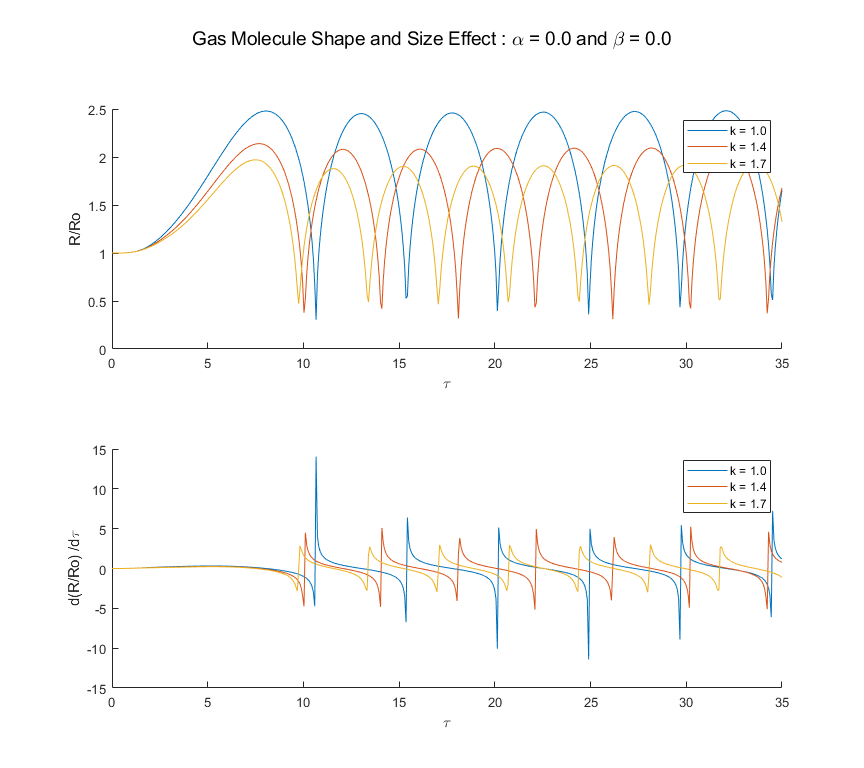
\includegraphics[width=0.90\textwidth]{./matlab/growingBubbles_MoleculeShapeSize.png}
	\caption{Gas molecule shape and size effect}
	\label{img:growingBubblesMoleculeShape}
\end{figure}

\begin{figure}[h!]
	\centering
	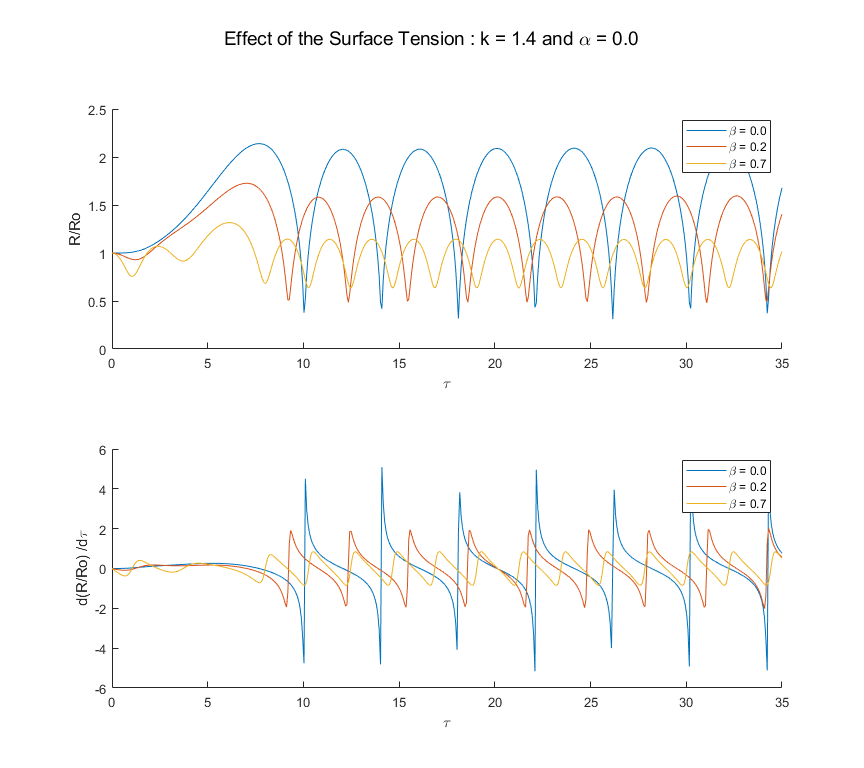
\includegraphics[width=0.90\textwidth]{./matlab/growingBubbles_SurfaceTension.png}
	\caption{Effect of the surface tension}
	\label{img:growingBubblesSurfaceTension}
\end{figure}

\begin{figure}[h!]
	\centering
	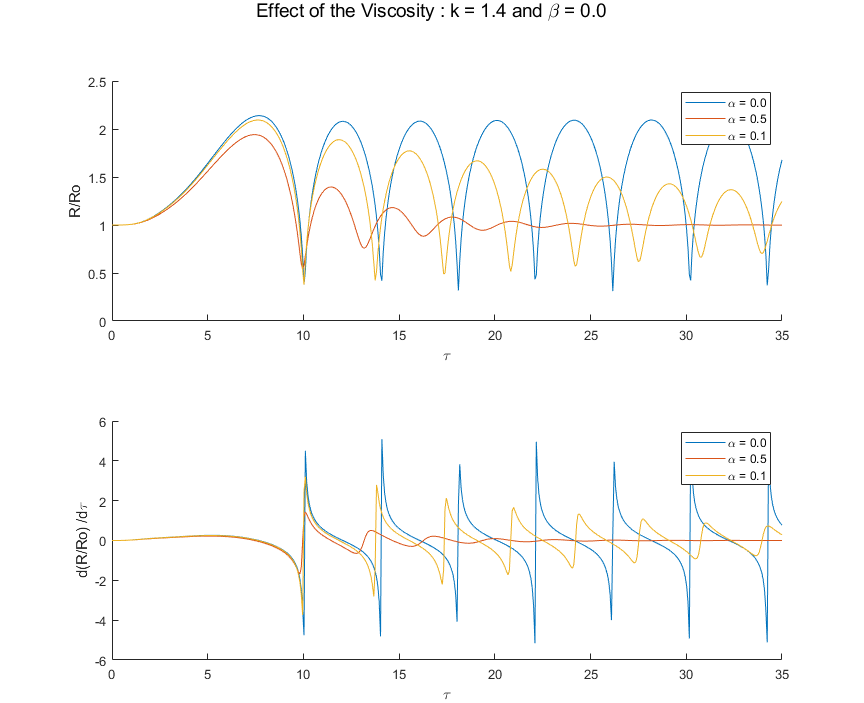
\includegraphics[width=0.90\textwidth]{./matlab/growingBubbles_Viscosity.png}
	\caption{Effect of the viscosity}
	\label{img:growingBubblesViscosity}
\end{figure}


\section{Part C : Draining Tank}

\begin{figure}[h!]
	\centering
	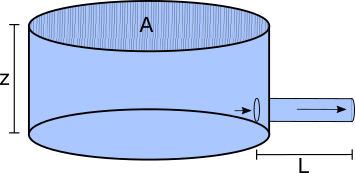
\includegraphics[width=0.40\textwidth]{./img/drainingTank.png}
	\caption{Effect of the viscosity}
	\label{img:drainingTank}
\end{figure}

For a tank (as in Figure \ref{img:drainingTank}), filled with an invisid fluid (no ciscous effect), the fluid height $z$ can be tracked with two equations: conservation of mass $\displaystyle - \dot{m}$ and conservation of energy $\displaystyle \frac{\ud (k + \Phi)}{\ud t}$.

$$ \frac{\ud m}{\ud t} = - \dot{m} = \frac{\ud}{\ud t} \left( \rho A z \right) $$
$$ - \dot{m} = \rho A \frac{\ud z}{\ud t} $$

$$ \frac{\ud (k + \Phi)}{\ud t} = - \dot{m} \left( \frac{1}{2} v^2 + g z \frac{p_0}{p} \right) $$
$$ \frac{\ud}{\ud t} \int \left[ \frac{1}{2} \rho A v^2 \ud z + \frac{1}{2} \rho A_0 {v_0}^2 \ud L + \rho A g z \ud z \right] = - \dot{m} \left( \frac{1}{2} {v_0}^2 \right) $$
$$ \frac{1}{2} \rho A v^2 \frac{\ud z}{\ud t} + \frac{1}{2} \rho z A \frac{\ud v^2}{\ud t} + \frac{1}{2} \rho A_0 L \frac{\ud {v_0}^2}{\ud t} + \rho A g z \frac{\ud z}{\ud t} = - \dot{m} \left( \frac{1}{2} {v_0}^2  \right) $$
$$ \rho A \frac{\ud z}{\ud t} \left[ \frac{1}{2} v^2 + g z + z v \frac{\ud v}{\ud z} + L \frac{A_0}{A} v_0 \frac{\ud v_0}{\ud z} \right] = - \dot{m} \left( \frac{1}{2} {v_0}^2  \right) $$
$$ \rho A \frac{\ud z}{\ud t} = - \rho v_0 A_0 $$
$$ A \frac{\ud z}{\ud t} = - v A $$
$$ \frac{\ud z}{\ud t} = - v $$
$$ \frac{1}{2} v^2 + g z + z v \frac{\ud v}{\ud z} + L \frac{A_0}{A} v_0 \frac{\ud v_0}{\ud z} = - \frac{1}{2} {v_0}^2 $$

Therefore the equation to solve is:

$$ \frac{\ud^2 z}{\ud t^2} = \frac{- g z + \left( \frac{\ud z}{\ud t} \right)^2 \frac{\lambda^4 - 1}{2}}{L \lambda^2 + z} $$
$$ \lambda = \frac{D}{D_0} $$
$$ \lambda^2 = \frac{A}{A_0} $$

where,

$$ y_1 = z $$
$$ y_2 = \frac{\ud z}{\ud t} = \frac{\ud y_1}{\ud t} $$

The ODEs to solve are:
$$ \frac{\ud y_2}{\ud t} = \frac{- g y_1 + {y_2}^2 \frac{\lambda^4 - 1}{2}}{L \lambda^2 + y_1} $$
$$ \frac{\ud y_1}{\ud t} = y_2 $$

with the following initial conditions:
$$ y_1 \rvert_{t = 0} = 1 \textrm{m} $$
$$ y_2 \rvert_{t = 0} = 1 \textrm{m/s} $$

Listing \ref{lis:drainingTankSolveAndPlot} solves and plot the previous ODEs.

\begin{lstlisting}[language=Matlab, caption=Draining Tank : Solve and Plot, label=lis:drainingTankSolveAndPlot]
% Runge-Kutta
g      = 9.81; % gravity
lambda = 10;   % Area/Area0
L      = 2;    % length of the pipe

% Plot
figure;
solveNplot_drainingTank(g, lambda, L, '')
suptitle(sprintf('Draining Tank : g = %1.1f, A/A_{0} = %1.1f, and L = %1.1f', g, lambda, L))

function[] = solveNplot_drainingTank(g, lambda, L, curveLabel)
    tspan = linspace(0, 50, 500);
    y1    = 1; % initial height (1m)
    y2    = 0; % initial velocity (0m/s)
    yo    = [y1, y2]';

    % Solve differential equation (medium order method)
    par(1) = g;
    par(2) = lambda;
    par(3) = L;
    [t, Y] = ode45(@drainingTank, tspan, yo, [], par);
    time   = t;
    Yout   = Y;

    %% Plot
    % Display radius vs. time
    hold all
    plot(time, Yout(:,1), 'DisplayName', curveLabel);
    xlabel('\tau');ylabel('z/z_o');
    %legend
end
\end{lstlisting}

\begin{figure}[h!]
	\centering
	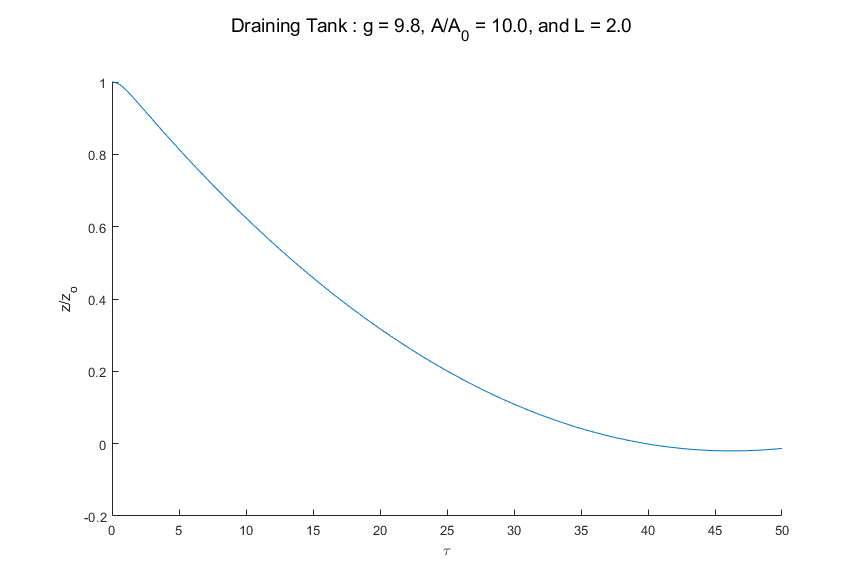
\includegraphics[width=0.90\textwidth]{./matlab/drainingTank_Height.png}
	\caption{Draining Tank Height $z$}
	\label{img:drainingTankHeight}
\end{figure}

As depicted in Figure \ref{img:drainingTankHeight}, the tank shall be emptied by time $\tau = 45$.

%\section{Part D : Introduction to Fluid Kinematics (ANSYS-Fluent) \cite{ANSYSmodelWing}}

\pagebreak 
\section*{Appendix}

\begin{lstlisting}[language=Matlab, caption=drainingTank]
function[ydot] = drainingTank(x, y, par)
    g      = par(1);
    lambda = par(2);
    L      = par(3);
    
    ydot(1) = y(2);
    ydot(2) = (-g*y(1) + ((y(2))^2*(lambda^4 - 1))/2) / (L*lambda^2  + y(1));
    ydot    = ydot';
end
\end{lstlisting}

\begin{lstlisting}[language=Matlab, caption=growingBubbles]
function[ydot] = growingBubbles(x, y, par)
    k   = par(1);
    a1  = par(2);
    b1  = par(3);
    tau = x;
    B   = (1+cos(pi*tau/5))/2;
    if tau > 10
        B = 1;
    end
    
    ydot(1) = y(2);
    ydot(2) = (-B+1/(y(1))^(3*k)-(3/2)*y(2)^2-a1*y(2)/y(1)-b1/y(1))/y(1);
    ydot    = ydot';
end
\end{lstlisting}

\begin{lstlisting}[language=Matlab, caption=reactub2]
%% TUBULAR REACTOR adapted from (jose lopez salinas)'s solution
function yprime = reactub_2(t, y, p)
    c  = y;           % Concentration in kmol/m3 of 'A'
    D  = p(1);        % Diffusion coefficient D
    k  = p(3);        % First order kinetic coefficient
    vo = p(4);        % Velocity of fluid injection
    N  = p(5);        % Number of nodes
    m  = 1;           % Chemical decomposition kinetics is first order
    dx = 1 / (N - 1); % Step size
    
    % Initially filled with an inert solvent
    yprime    = zeros(1, N-1);
    yprime(1) = 0;
    
    % centered differences with truncation error proportional to the step
    % size to the power 2
    for i = 2 : N - 1
        sum0 = D * (c(i + 1) - 2 * c(i) + c(i - 1)) / (dx^2);
        sum1 = vo * (c(i + 1) - c(i - 1)) / (2 * dx);
        sum2 = k * c(i)^m;
        yprime(i) = sum0 - sum1 - sum2;
    end
    for i = N : -1 : 2
        yprime(N) = (4 * yprime(N - 1) - yprime(N - 2)) / 3;
    end
    yprime = yprime';
end
\end{lstlisting}

\begin{lstlisting}[language=Matlab, caption=reactub3]
%% TUBULAR REACTOR adapted from (jose lopez salinas)'s solution
function yprime = reactub_3(t, y, p)
    c  = y;           % Concentration in kmol/m3 of 'A'
    D  = p(1);        % Diffusion coefficient D
    k  = p(3);        % First order kinetic coefficient
    vo = p(4);        % Velocity of fluid injection
    N  = p(5);        % Number of nodes
    m  = 1;           % Chemical decomposition kinetics is first order
    dx = 1 / (N - 1); % Step size
    
    % Initially filled with an inert solvent
    yprime    = zeros(1, N-1);
    yprime(1) = 0;
    
    % centered differences with truncation error proportional to the step
    % size to the power 2
    for i = 2 : N - 1
        sum0 = D * (c(i + 1) - 2*c(i) + c(i - 1)) / (dx^2);
        sum1 = vo * (c(i + 1) - c(i - 1)) / (2*dx);
        sum2 = k * c(i)^m;
        yprime(i) = sum0 - sum1 - sum2;
    end
    
    for i = N : -1 : 3
        yprime(N) = (yprime(N - 3) - 4*yprime(N - 2) + 5*yprime(N - 1)) / 2;
    end
    yprime = yprime';
end
\end{lstlisting}

\begin{lstlisting}[language=Matlab, caption=reactub4]
%% TUBULAR REACTOR adapted from (jose lopez salinas)'s solution
function yprime = reactub_4(t, y, p)
    c  = y;           % Concentration in kmol/m3 of 'A'
    D  = p(1);        % Diffusion coefficient D
    k  = p(3);        % First order kinetic coefficient
    vo = p(4);        % Velocity of fluid injection
    N  = p(5);        % Number of nodes
    m  = 1;           % Chemical decomposition kinetics is first order
    dx = 1 / (N - 1); % Step size
    
    % Initially filled with an inert solvent
    yprime    = zeros(1, N-1);
    yprime(1) = 0;
    
    % centered differences with truncation error proportional to the step
    % size to the power 2
    for i = 2 : N - 1
        sum0 = D * (c(i + 1) - 2*c(i) + c(i - 1)) / (dx^2);
        sum1 = vo * (c(i + 1) - c(i - 1)) / (2*dx);
        sum2 = k * c(i)^m;
        yprime(i) = sum0 - sum1 - sum2;
    end
    
    for i = N : -1 : 4
        yprime(N) = (-3*yprime(N - 4) + 14*yprime(N - 3) - 24*yprime(N - 2) + 18*yprime(N - 1)) / 5;
    end
    yprime = yprime';
end
\end{lstlisting}

\printbibliography[title={References}]
\end{document}
